\section{Final time intervals at matched resolution}\label{sec:matched}
Both independent methods use the same number of radial cells and the same
maximum time step in each comparison. We first halve the step at 320 liner
cells (5 to 2.5~ms), then double the liner mesh to 640 cells at 2.5~ms.
The casing has one quarter the liner cell count. All runs impose the same
continuous nominal heating and evolve the casing from ambient temperature.

\begin{center}\small\begin{tabular}{lrrrrr}\toprule
& Fine FV & Fine nodal & FV time-step & FV mesh & Final gap\\
Motor & [s] & [s] & change [ms] & change [ms] & [ms]\\\midrule
Sustainer Al & 110.4763 & 110.4822 & +0.35 & -2.10 & 3.62 \\
Sustainer CF & 104.2531 & 104.2571 & -0.11 & -1.93 & 1.71 \\
Booster Al & 147.6159 & 147.6233 & +0.86 & -3.85 & 5.10 \\
Booster CF & 137.9460 & 137.9505 & -0.10 & -2.84 & 2.28 \\
\bottomrule\end{tabular}\end{center}
The time columns give the upper ends of the last integration intervals. Each
change column subtracts the previous finite-volume endpoint while varying
just the indicated setting. At the finest common resolution, the largest
difference between method endpoints is 7.35~ms. At common half-second stations,
the largest thickness difference is 0.23~$\mu$m and the largest casing-interface
temperature difference is 0.17~K.

\begin{figure}[H]\centering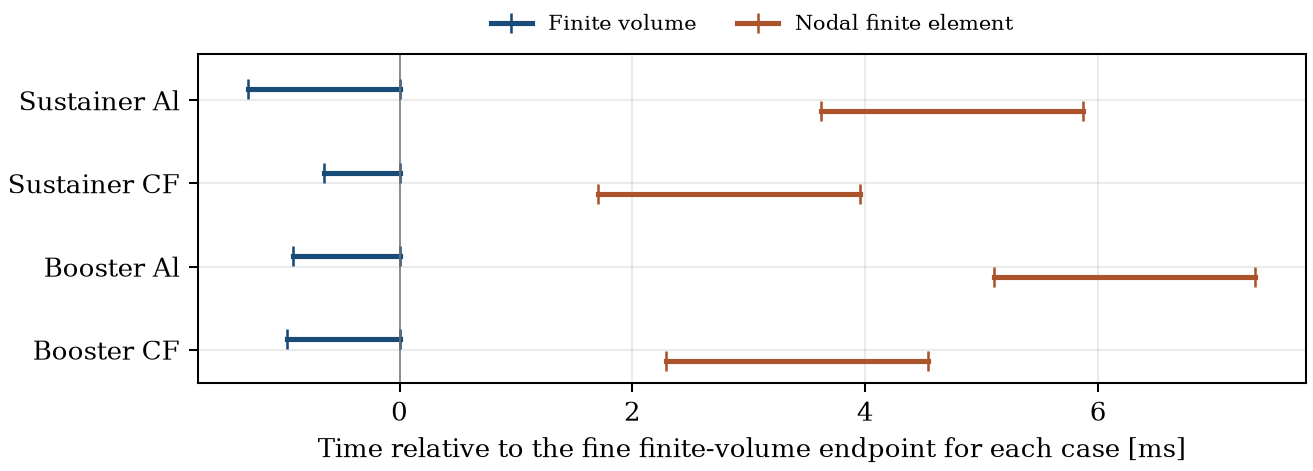
\includegraphics[width=.96\textwidth]{../analysis/matched_final_intervals.png}
\caption{Each segment runs from the last saved step with liner present to the
numerical exhaustion event. The origin in each row is its own FV endpoint.
The clear space between segments is the gap reported in the table.}
\end{figure}
The final numerical intervals are separated in all four cases.
Their width reflects the integration step alone. The unknown firing heat flux,
recession chemistry and post-limit casing response introduce separate physical
uncertainties.

\paragraph{Output-time recovery.}
One FV run approached the 142~s sample to about $1.0\times10^{-10}$~s and
attempted a separate step of that duration. Its energy check rejected the step.
The successor splits the preceding interval into two comparable steps whenever
the next sample would otherwise leave a remainder below 5\% of a normal step.
It resumed the Al booster from its saved 126.235~s state, retaining its mass and
heat histories. The seven already completed FV paths kept their original
records. All twelve comparisons use the original balance tolerances.
\clearpage
